% !TEX root=../main.tex
\section{Tutorial}
\subsection{Трехмерный гармонический осциллятор}
Полная энергия $E = E_x + E_y + E_z$.
Остальная инфа в \eqref{eq:psi_free-main-results}.
Считаем число состояний:
\begin{equation}
    \label{eq:3d-harmonic-number_of_states}
    \mathcal{N}(E)=
    \sum_{E_{x}=0}^{E}\left\{\begin{array}{c}\text { number of choices } \\ \text { for } E_{y} \text { given } E_{x}\end{array}\right\}=
    \sum_{E_{x}=0}^{E}\left(E-E_{x}+1\right) =
    \frac{(N+1)(N+2)}{2}
\end{equation}

Записываем через дельту Кронекера:
\begin{equation}
    \label{eq:3d-harmonic-number_of_states-kroneker}
    \mathcal{N}(E)=\sum_{E_{x}=0}^{E} \sum_{E_{y}=0}^{E} \sum_{E_{z}=0}^{E} \delta_{\left(E_{x}+E_{y}+E_{z}\right), E}
\end{equation}

А затем вспоминаем, что дельту можно представить через интеграл:
\begin{equation}
    \label{eq:kroneker_delta-integral}
    \delta_{j, k}=\int_{-\pi}^{\pi} \frac{d \lambda}{2 \pi} e^{i(j-k) \lambda}
\end{equation}

Впихиваем в \eqref{eq:3d-harmonic-number_of_states} и считаем геометрическую прогрессию:
\begin{align}
    \label{eq:3d-harmonic-number_of_states-via-integral}
    & \mathcal{N}(E)=\int_{-\pi}^{\pi} \frac{d \lambda}{2 \pi} e^{-i E \lambda}\left(\sum_{E_{x}=0}^{E} e^{i E_{x} \lambda}\right)\left(\sum_{E_{y}=0}^{E} e^{i E_{y} \lambda}\right)\left(\sum_{E_{z}=0}^{E} e^{i E_{z} \lambda}\right) \\
    & \mathcal{N}(E)=\int_{-\pi}^{\pi} \frac{d \lambda}{2 \pi} \underbrace{e^{-i E \lambda}\left[\frac{1-e^{i(E+1) \lambda}}{1-e^{i \lambda}}\right]^{3}}_{\mathcal{N}(E, \lambda)}
\end{align}

Подстановка $e^{i\lambda} = z$ сводит интеграл к комплексному, который можно взять по т. Коши о вычетах.
Разминайтесь с ТФКП-ом сами, результат будет такой же, как и \eqref{eq:3d-harmonic-number_of_states}.

\subsection{Неразличимость частиц}
Рассмотрим все состояния с $E \leq 4$ и рассмотрим соответствующие ей $35$ ($15+10+6+3+1$) состояний (рис. \ref{fig:35-states-example}).
Основная проблема, с которой нам придется бороться --- это неразличимость частиц.
Это значит, что состяния на рисунке \ref{fig:indistinguishable-states-example} все одинаковы и в статсумме $Z$ \textbf{их надо считать только один раз}.

\begin{figure}[ht]
    \begin{subfigure}{0.33\columnwidth}
        \centering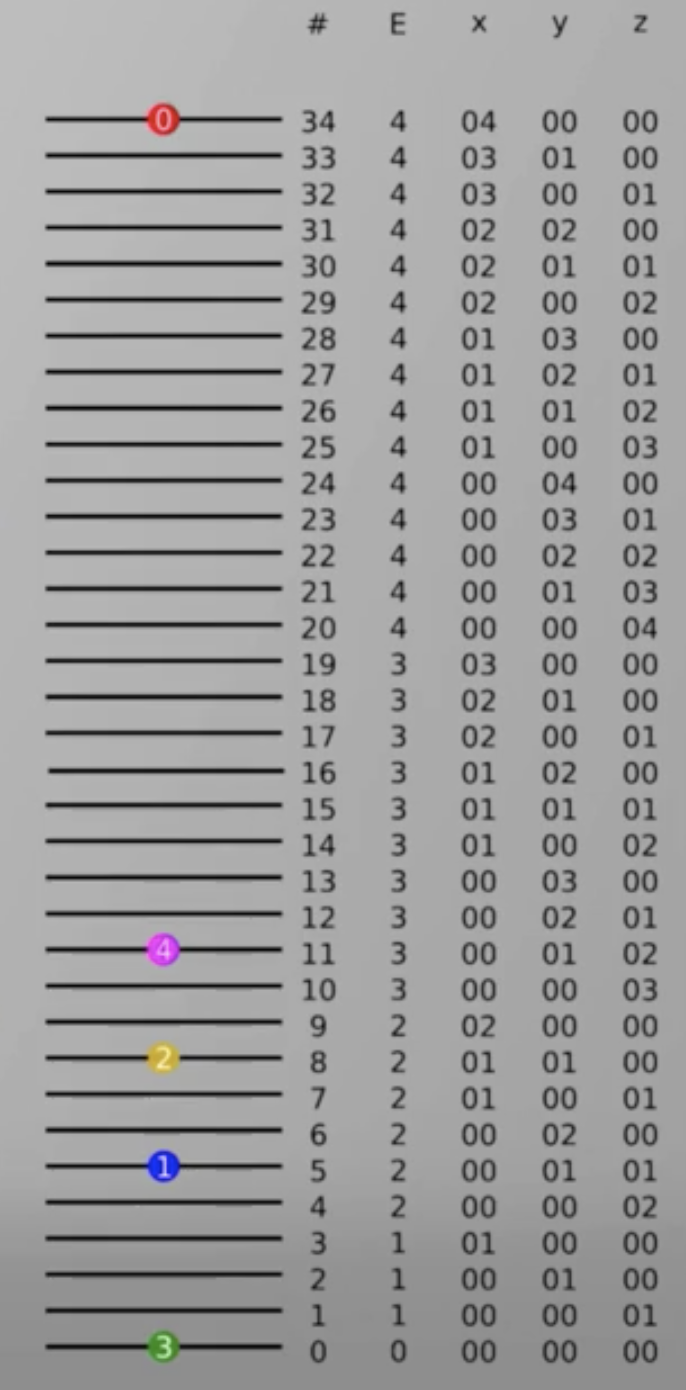
\includegraphics[width=\linewidth]{fig/35-states}
        \caption{35 состояний для бозонов}
        \label{fig:35-states-example}
    \end{subfigure}
    \begin{subfigure}{0.66\columnwidth}
        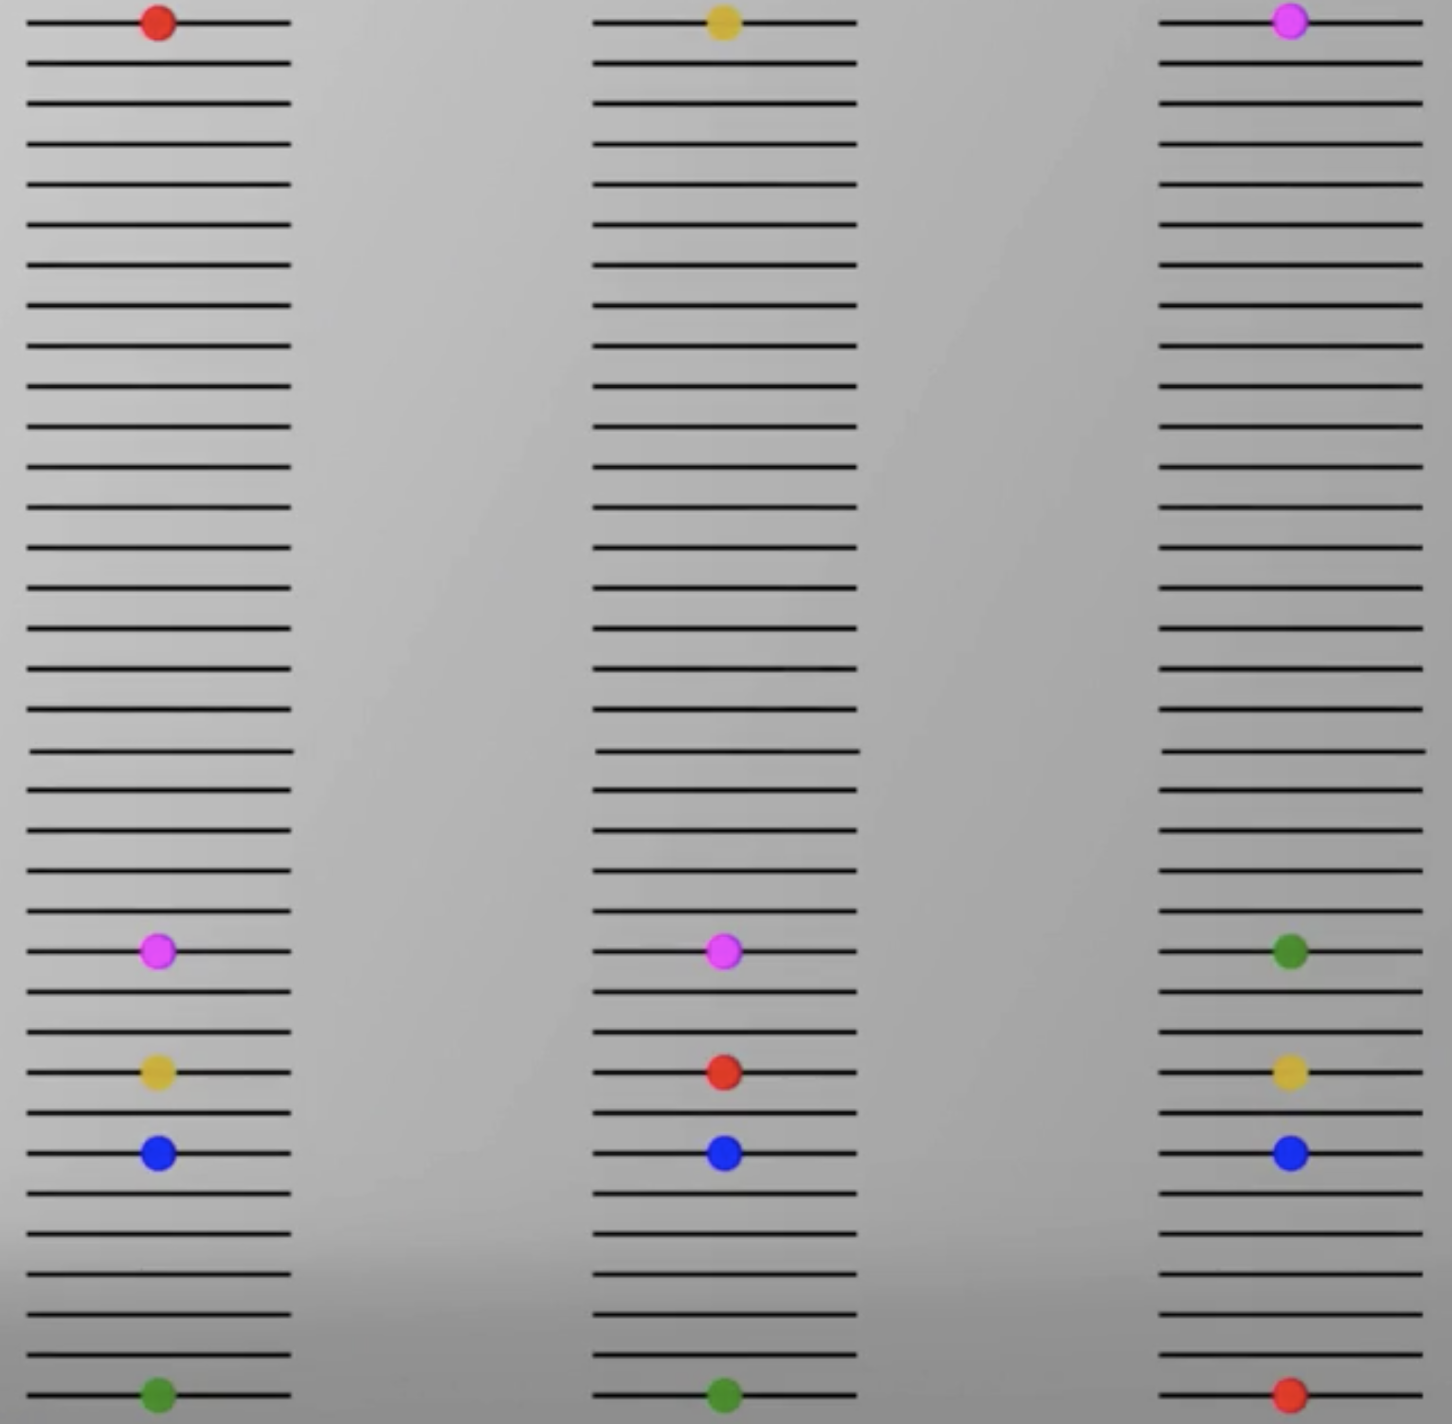
\includegraphics[width=\linewidth]{fig/indistinguishable-states}
        \caption{Три неразличимые конфигурации}
        \label{fig:indistinguishable-states-example}
    \end{subfigure}
    \caption{К подсчету числу состояний бозонов}
\end{figure}

Чтобы решить проблема повторного подсчета, мы будем учитывать только состояния, в котором состояние частицы 0 $\sigma_0$ ниже состояния частицы 1 $\sigma_1$, т.е. $\sigma_0 \leq \sigma_1 \leq \dots \leq \sigma_N$.
В нашем случае: $0 \leq \sigma_{0} \leq \sigma_{1} \leq \sigma_{2} \leq \sigma_{3} \leq \sigma_{4} \leq 34$.

Этот трюк позволяет считать статсумму для бозонов, считая по факту их различимыми.
Для этого берем частицу 0 и сажаем ее в любое состояние $\sigma_0 \in [0, 34]$, затем берем частицу 1 и сажаем ее в любое состяние между частицей 1 и 34 $\sigma_1 \in [\sigma_0, 34]$ и так далее, пока не посадим всех (рис. \ref{fig:putting-particles}).

Это порождает формулу:
\begin{equation}
    \label{eq:Z_E-via-sigmas}
    Z(\beta)=\sum_{0 \leq \sigma_{0} \leq \ldots \leq \sigma_{4} \leq 34} e^{-\beta E\left(\sigma_{0}, \ldots, \sigma_{4}\right)}
\end{equation}
и алгоритм \ref{code:naive_boson_trap}.
\pythonfile{../w6/programs_tutorial_6/naive_boson_trap}{Подсчет $Z$ через сумму по $\sigma$ (\texttt{naive\_boson\_trap.py})}{code:naive_boson_trap} 

\begin{figure}[ht]
    \begin{subfigure}{0.33\columnwidth}
        \centering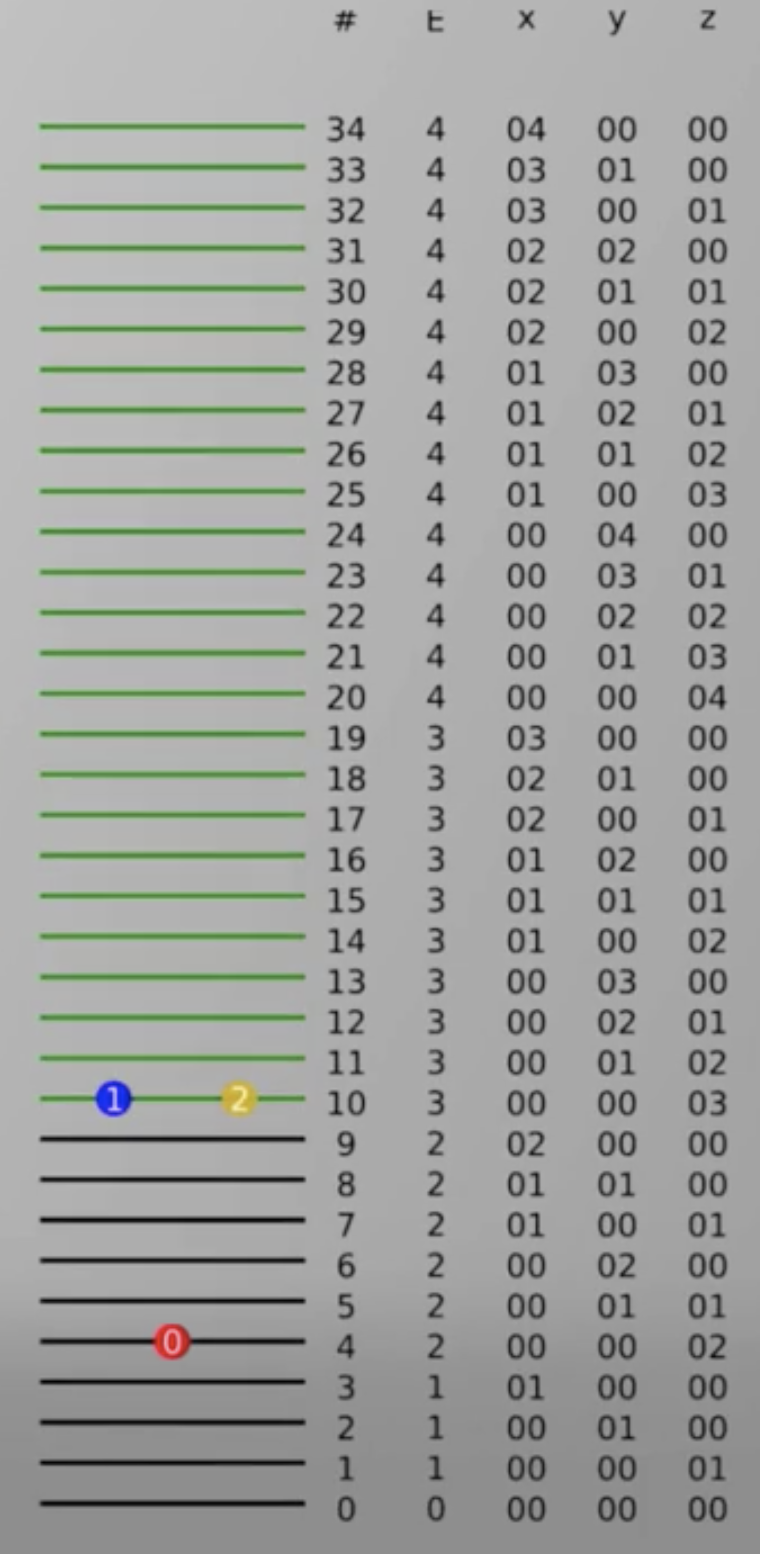
\includegraphics[width=\linewidth]{fig/putting-particles}
        \caption{Расстановка 5 частиц как будто бы они различимы}
        \label{fig:putting-particles}
    \end{subfigure}
    \begin{subfigure}{0.33\columnwidth}
        
\includegraphics[width=0.8\linewidth, height=2\linewidth]{fig/balls-walls}
        \caption{Сведение к задаче о шариках и стенках}
        \label{fig:balls-walls}
    \end{subfigure}
    \caption{К подсчету числу состояний бозонов}
\end{figure}

Как же подсчитать суммарное число расстановок бозонов?
Очень просто: мы сводим задачу к шарикам и стенкам (надеюсь, узнаете), где шарики --- это бозоны, а стенок $35+5-1=39$ штук (см. рисунок \ref{fig:balls-walls}).
Тогда число расстановок бозонов равно числу расстановок шариков в такой системе: $\cfrac{39!}{4!35!} = 575757$.

Введем \textit{число заполнения} $\{n_0, n_1, \dots, n_{34}\}$ --- сколько частиц лежит на каждом уровне.
Тогда полная энергия состояния запишется как $E_{\text{tot}} = n_0 E_0 + n_1 E_1 + \dots n_{34} E_{34}$.
Подсчитаем статсумму, воспользовавшись дельтой Кронекера в интегральном представлении:
\begin{align}
    \label{eq:Z-5_particles-via-delta}
    & Z(\beta)=\sum_{n_{0}=0}^{5} \cdots \sum_{n_{34}=0}^{5} e^{-\beta\left(n_{0} E_{0}+\ldots+n_{34} E_{34}\right)} \delta_{\left(n_{0}+\ldots+n_{34}\right), 5}, 
    & \left(\delta_{j, k}=\int_{-\pi}^{\pi} \frac{d \lambda}{2 \pi} e^{i(j-k) \lambda}\right) \\
    & Z(\beta)=\int_{-\pi}^{\pi} \frac{d \lambda}{2 \pi} e^{-i N \lambda} \underbrace{\left(\sum_{n_{0}} e^{n_{0}\left(-\beta E_{0}+i \lambda\right)}\right)}_{f_{0}(\beta, \lambda)} \ldots \underbrace{\left(\sum_{n_{34}} e^{n_{34}\left(-\beta E_{34}+i \lambda\right)}\right)}_{f_{34}(\beta, \lambda)} &
\end{align}

Пределы суммирования здесь идут до $N$, однако можно взять $N\rightarrow \infty$ и сократить по формуле:
\begin{align}
    \label{eq:upsilon-geometrical}
    & |\Upsilon|=\left|e^{-\beta E} e^{i \lambda}\right|=\underbrace{\left|e^{-\beta E}\right|}_{\leq 1 \atop E>0} \underbrace{\left|e^{i \lambda}\right|}_{1} \\
    \nonumber
    & \sum_{n=0}^{N} \Upsilon^{n}=\frac{1-\Upsilon^{N+1}}{1-\Upsilon} \quad \frac{N \rightarrow \infty}{|\Upsilon|<1} \quad \frac{1}{1-\Upsilon} \\
    \nonumber
    & f_{E}(\beta, \lambda) =\frac{1-\exp [i(N+1) \lambda]}{1-\exp (i \lambda)}, \quad E=0, \quad \text {(ground state)}\\
    \nonumber
    & f_{E}(\beta, \lambda) =\frac{1}{1-\exp (-\beta E+i \lambda)}, \quad E>0, \quad(\text {excited state})
\end{align}

Здесь $f_E (\beta, \lambda)$ в ground state получено применением суммы геометрической прогрессии \textit{до конечного $N$}.
Этот подход несколько <<наивен>> и в будущем мы применим ТФКП для нормального рассмторения.

\begin{wrapfigure}[10]{r}{0.3\linewidth}
    \label{fig:N_0-T-plot}
    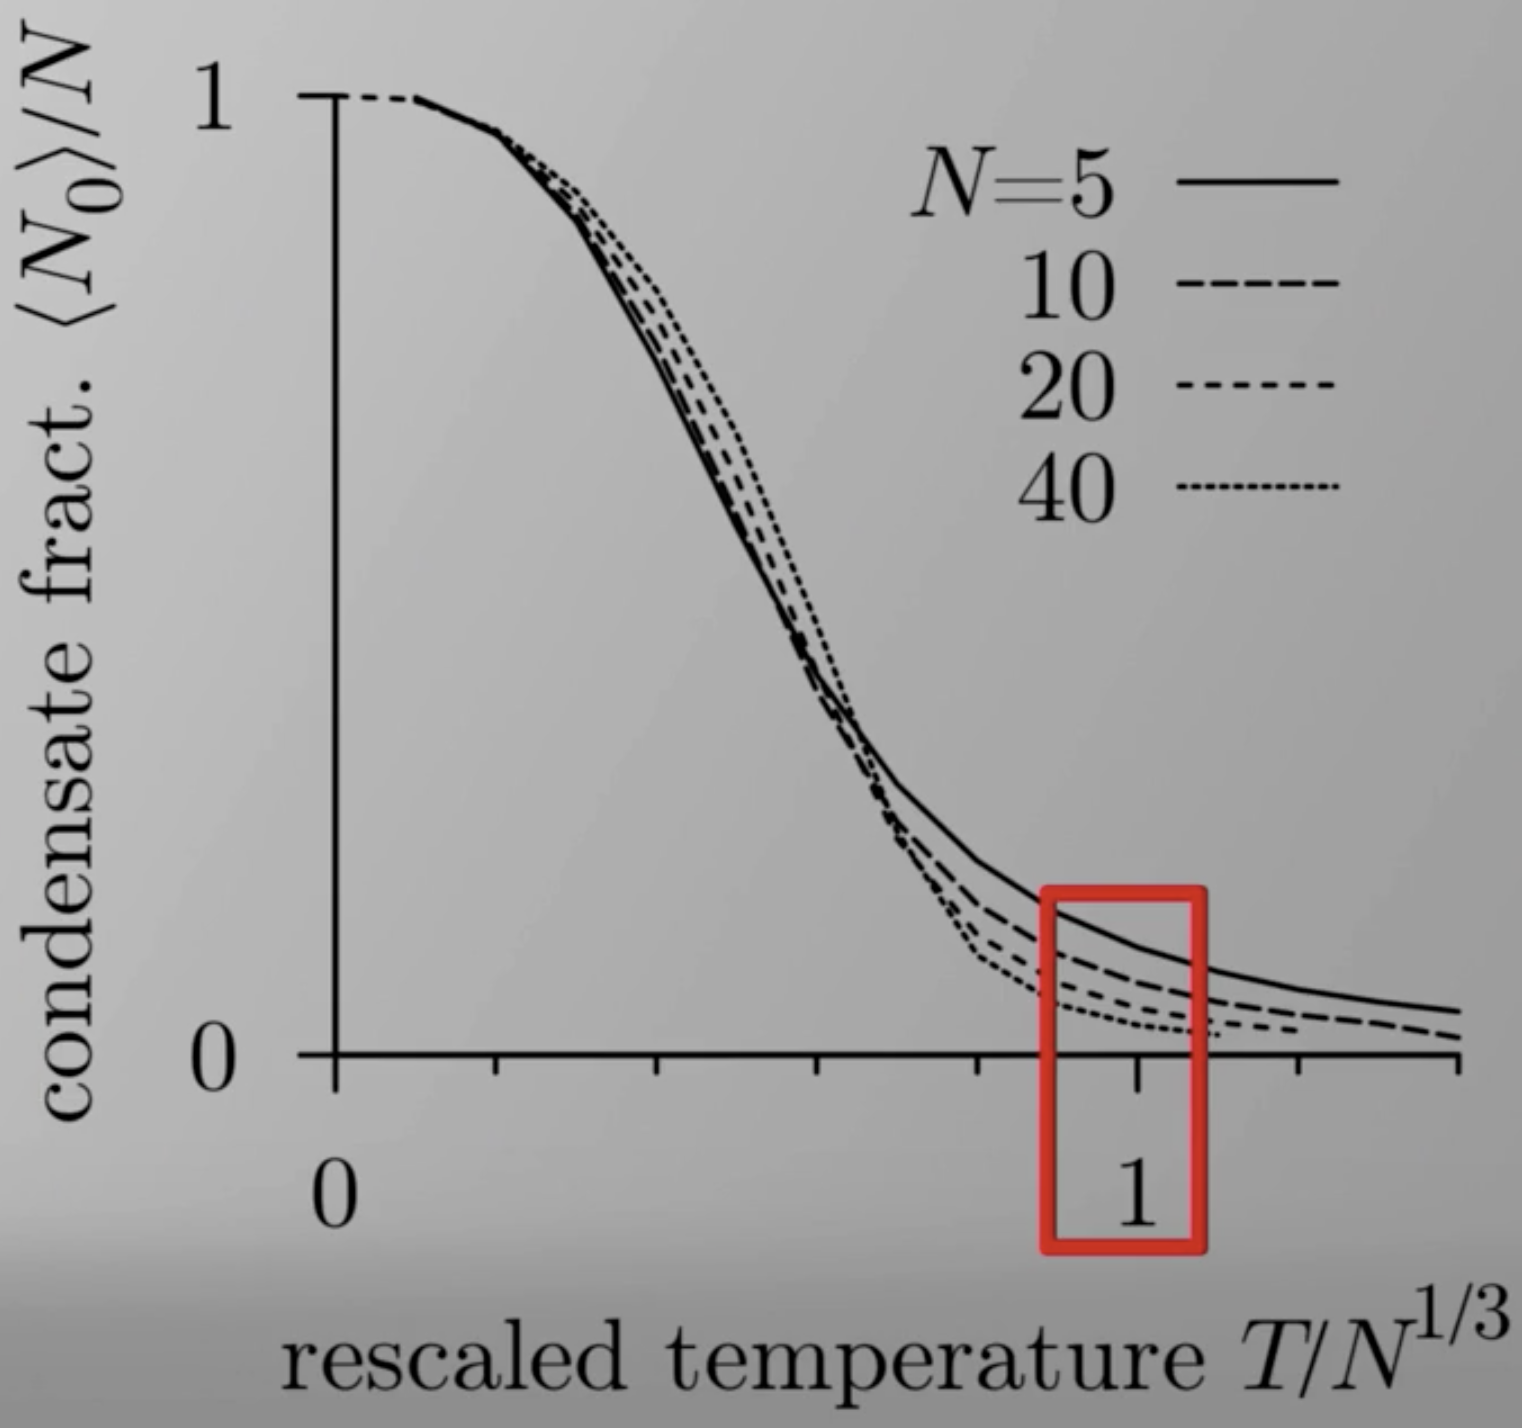
\includegraphics[width=\linewidth]{fig/N_0-T-plot}
    \caption{Зависимость $\braket{N_0}$ от температуры (удельные единицы)}
\end{wrapfigure}

После суммирования \eqref{eq:upsilon-geometrical} можно получить статсумму:
\begin{equation}
    \label{eq:bosons-partition-function}
    Z_{N}(\beta)=\int_{-\pi}^{\pi} \frac{\mathrm{d} \lambda}{2 \pi} \underbrace{\mathrm{e}^{-\mathrm{i} N \lambda} \prod_{E=0}^{E_{\max }}\left[f_{E}(\beta, \lambda)\right]^{\mathcal{N}(E)}}_{Z_{N}(\beta, \lambda)}
\end{equation}
где $\mathcal{N}(E)$ --- число уровней для заданной энергии $E$ (например, $\mathcal{N} (E_{34}) = 34$).

Используя статсумму, можно подсчитать, например, число частиц на нулевом уровне энергии:
\begin{align}
    \label{eq:bosons-N_0-mean}
    & N_{0}(\beta, \lambda)=\frac{\partial}{i \partial \lambda} f_{0}=\left[-\frac{(N+1) e^{i \lambda(N+1)}}{1-e^{i \lambda(N+1)}}+\frac{e^{i \lambda}}{1-e^{i \lambda}}\right] \\
    & \braket{N_{0}(\beta)}=\frac{1}{Z_{N}(\beta)} \int_{-\pi}^{\pi} \frac{d \lambda}{2 \pi} e^{-i N \lambda} N_{0}(\beta, \lambda) \prod_{E=0}^{E_{\max }}\left[f_{E}(\beta, \lambda)\right]^{\mathcal{N}(E)}
\end{align}

Можно из \eqref{eq:bosons-N_0-mean} получить Бозе-конденсацию, рассматривая график для $\braket{N_0}$ (рис. \ref{fig:N_0-T-plot}).
